\subsection{Vehicle Model}

\begin{frame}{Vehicle Properties}
\begin{itemize}
\item Instantaneous change in velocity
\item Constant velocity within intersection
\item Velocity (MPH): $V \rightarrow V \in [20,40]$
\item Route intention constant throughout intersection traversal
\item Randomized vehicle entry times
\item Receives velocity change or delayed start time from controller
\end{itemize}
\end{frame}

\begin{frame}{Modeling Tool}
\begin{center}
Ptolemy II Version 8.0.1

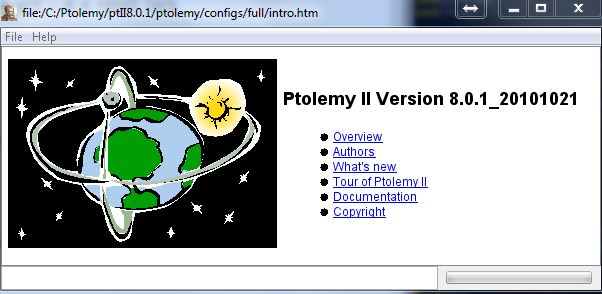
\includegraphics[scale=0.5]{diagram/ptolemy.jpg}
\end{center}
\end{frame}

\begin{frame}{Intersection Model}
\centering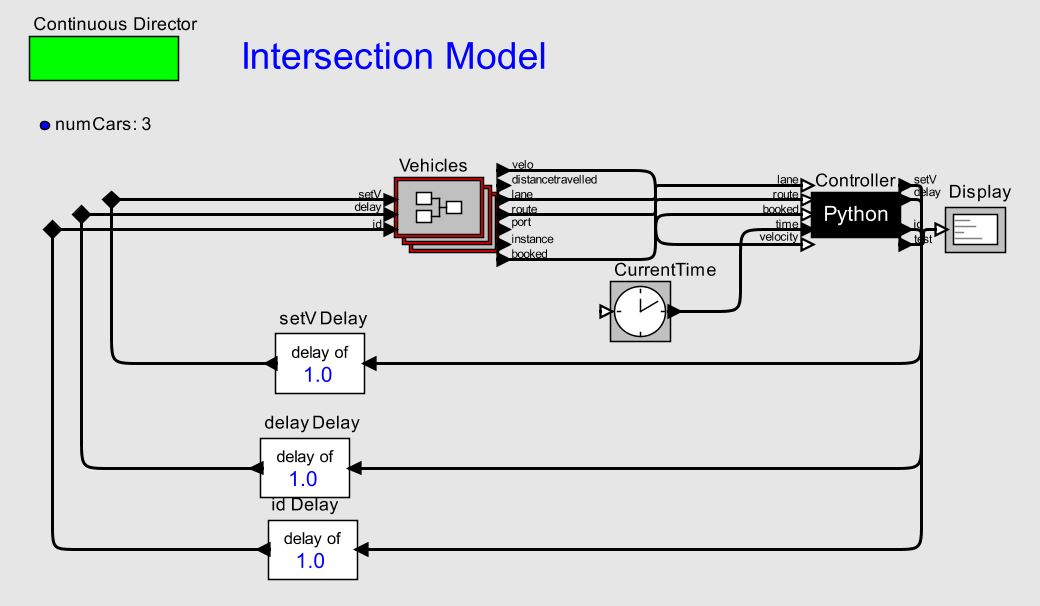
\includegraphics[width=0.9\linewidth]{diagram/ptolemy_system.jpg}
\end{frame}

\begin{frame}{Modeling Continuous Vehicle Flow}
Ptolemy limitations prevent dynamic instantiation of actors.
\begin{block}{Multi-Instance Composite Actor}
\begin{minipage}{0.45\linewidth}
\begin{itemize}
\item Vehicle instances accessed by ID encoding
\item Create $N$ vehicle Modal Model instances
\item Generate random:
	\begin{itemize}
	\item Intersection entry time: $1-45$ seconds
	\item Initial velocity (m/s): $V_0 \in [20,40]$
	\item Direction: $N,S,E,W$
	\item Route: $L,S1,S2,R$
	\end{itemize}
\end{itemize}
\end{minipage}
\hfill
\begin{minipage}{0.45\linewidth}
\begin{itemize}
\item Implement as many instances of the car model as desired
\item Interacts with Python-based controller
\item Car can ``re-enter'' system only after it exits (re-use vehicles 
	vs. generating new vehicles)
\end{itemize}
\end{minipage}
\end{block}
\end{frame}

\begin{frame}{Vehicle Modeling}
\centering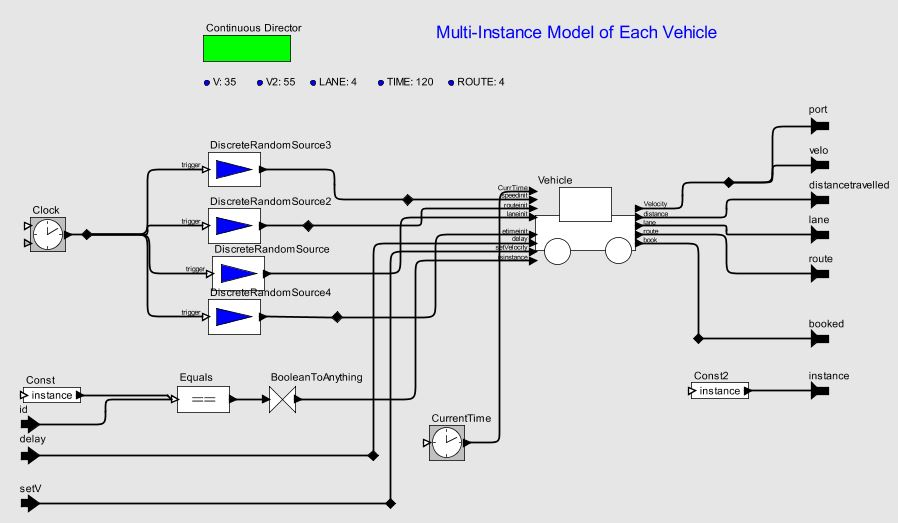
\includegraphics[width=0.9\linewidth]{diagram/ptolemy_multiinstance_actor.jpg}
\end{frame}

\begin{frame}{Vehicle States}
\begin{itemize}
\item $RUN$
\item $IDLE$
\item $ENTER$
\item $BOOK$
\item $GO$
\item $WAIT$
\end{itemize}
\end{frame}

\begin{frame}{Vehicle FSM Actor}
\centering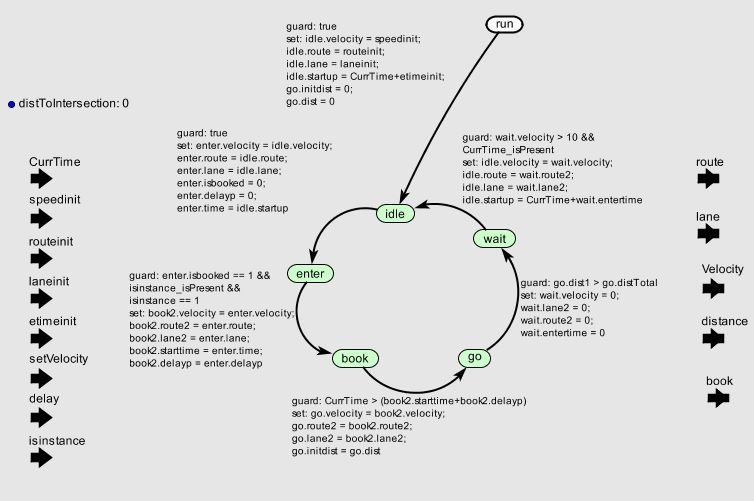
\includegraphics[width=0.9\linewidth]{diagram/ptolemy_vehicle_fsm.jpg}
\end{frame}

\begin{frame}{\texttt{ENTER} State}
Abstraction:
\begin{itemize}
\item Equivalent to pre-conflict entrance approach
\item Initial velocity used to calculate time until intersection
\item Stops at intersection if instructions not received from controller
\end{itemize}
Guard:
\begin{itemize}
\item $t_\text{GLOBAL} > t_\text{ENTER}$
\end{itemize}
\end{frame}

\begin{frame}{\texttt{ENTER} State}
\centering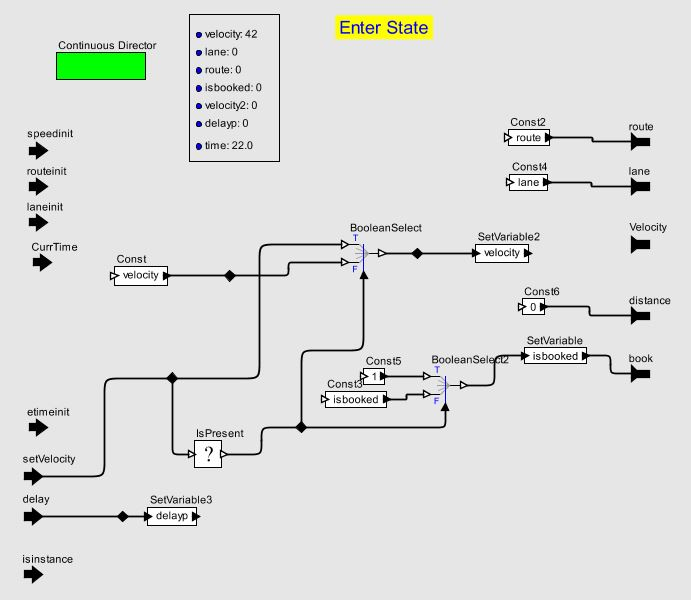
\includegraphics[width=0.7\linewidth]{diagram/ptolemy_vehicle_enter.jpg}
\end{frame}

\begin{frame}{\texttt{GO} State}
Abstraction:
\begin{itemize}
\item Equivalent to the approach through the intersection
\item Tracks when the vehicle leaves the system
\item Stops at intersection if instructions not received from controller
\end{itemize}
Guard:
\begin{itemize}
\item $t_\text{GLOBAL} > t_\text{STRAIGHTAWAY}$
\end{itemize}
\end{frame}

\begin{frame}{\texttt{GO} State}
\centering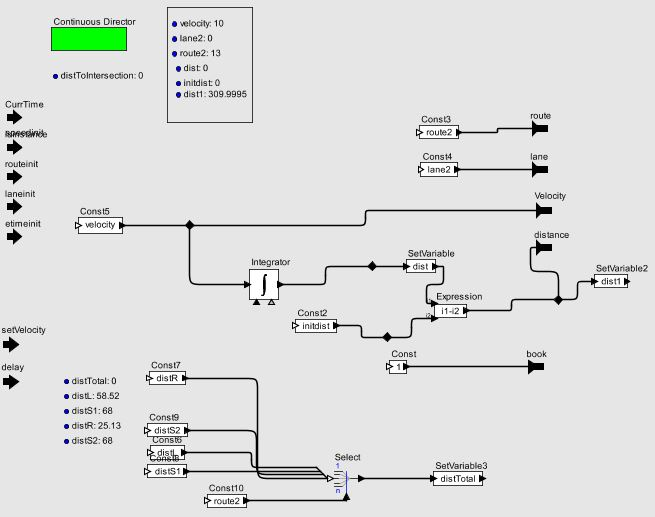
\includegraphics[width=0.75\linewidth]{diagram/ptolemy_vehicle_go.jpg}
\end{frame}

